% =====================================================================
%  ECC 2027 submission draft (ieeeconf, 6 pages; 8 allowed for review).
%  Deadline: 31 October 2026.
%  Plain English: short sentences, one idea each, every term defined.
%  Numbers marked % [NEW] are reproduced by the scripts listed in
%  scripts/README.md (reproduce.py, conv.py, twodof.py, noise.py,
%  designed.py, owner_designed.py, fig_stair.py, fig_record.py,
%  fig_certified.py).
% =====================================================================
\documentclass[letterpaper, 10 pt, conference]{ieeeconf}
\IEEEoverridecommandlockouts
\overrideIEEEmargins

\usepackage{amsmath,amssymb}
\usepackage{graphicx}
\usepackage{booktabs}
\usepackage{url}

\newtheorem{lemma}{Lemma}
\newtheorem{proposition}{Proposition}
\newtheorem{corollary}{Corollary}
\newenvironment{proof}{\noindent\textit{Proof:}\ }{\hfill$\square$\par\smallskip}
\usepackage{xspace}
\newcommand{\spin}{SPIN\xspace}

\title{\LARGE\bf Certified Robustness for Model-Free PID Tuning\\
by Step-Response Inspection}

% Author block taken from the SPIN paper -- confirm the list and order.
\author{Pavel Otta$^{1}$, Daniel Pachner$^{1}$, Ji\v{r}\'{\i} Dost\'al$^{1}$
and Vladim\'{\i}r Havlena$^{2}$%
\thanks{$^{1}$University Centre for Energy Efficient Buildings (UCEEB),
Czech Technical University in Prague, Bu\v{s}t\v{e}hrad, Czech Republic.
Corresponding author: {\tt pavel.otta@cvut.cz}}%
\thanks{$^{2}$Department of Control Engineering, Faculty of Electrical
Engineering, Czech Technical University in Prague, Czech Republic.}}

\begin{document}

\maketitle
\thispagestyle{empty}
\pagestyle{empty}

\begin{abstract}
The \spin method tunes a PID controller without a model. After each
setpoint step it counts how many turns the control error makes in three
phase portraits, and it raises the gains until one count is above its
limit. The limits were chosen by calibration, and nothing guaranteed the
robustness of the result. Our results are twofold. First, for tunings
that cancel the plant lags, the counts have an exact meaning. The loop has
one parameter $k$, its gain margin is $\pi/(2k)$, and the error crosses
the setpoint only if $M_s>1.39$. Each crossing adds exactly half a turn
to the count, so at the default settling band of $2\%$ a count of at most
half a turn guarantees $M_s\le1.53$, and each calibrated limit of \spin
turns out to separate $n$ from $n+1$ crossings. Second, for any stable loop, the
counts and $M_s$ are not tied in either direction, but the error after a
setpoint step is the step response of the sensitivity function. So the
step itself gives $M_s$, and the loop $L=1/S-1$, so it also predicts the
peak of any other tuning of the same plant. We use both as an acceptance
test and a shaping rule inside \spin: if the peak is too high, \spin
lowers the band whose move is predicted to help, and we prove when such a
band exists. On $19$ test loops and two start tunings, \spin as published
ended above $M_s=1.7$ on $8$ or $9$ loops, up to $2.07$, depending on the
start. With the rule, all $19$ loops ended at or below the target from
both starts, within a reading error below $1\%$, at a mean load-rejection
cost of $5$ to $8\%$. An ablation shows that the rule, not the gain box,
does this.
\end{abstract}

\section{Introduction}

Let $L=CG$ be the loop transfer function and $S=1/(1+L)$ the sensitivity
function. The peak $M_s=\max_\omega|S(j\omega)|$ measures robustness. A
value near $1.4$ is safe, and a value near $2$ is close to the limit
\cite{AstromHagglund2004}. Tuning rules reach a
chosen $M_s$ by using a model \cite{AstromHagglund2004,Skogestad2003}.
After tuning, plants rarely check $M_s$, because a check needs a model or
a test that disturbs production \cite{Desborough2002,Bauer2016}.

\subsection{The \spin method}

\spin \cite{SPIN} tunes a PI or PID controller $C(s)=K_p+K_i/s+K_ds$
without a model. In each iteration it applies one setpoint step and
records the control error $e$. From this record it forms three phase
portraits,
\begin{equation}
\Gamma_0:(e,z),\quad \Gamma_1:(\Delta e,e),\quad
\Gamma_2:(\Delta^2e,\Delta e),
\label{eq:portraits}
\end{equation}
where $z(t)=\int_0^te\,dt'$ is the running integral of $e$ and $\Delta$ is
the difference between samples. Each portrait reacts to one frequency band. The bands
belong to $K_i$, $K_p$ and $K_d$. The turn count $N_k$ is the number of
turns that $\Gamma_k$ makes around its end point before the error stays
within a band $\delta$ (by default $2\%$ of the step). Each count has a
limit $\bar N_k$, and Algorithm~1 gives the rule. An oscillation shows in
its own band and in all higher bands, so the lowest band above its limit
is the one that causes it. \spin needs no model, no identification and
no plant-specific setting: the same dimensionless defaults served every
plant in \cite{SPIN}. But the limits were chosen by calibration, and
nothing guaranteed the robustness of the result. This paper adds one
test to line 7 (Algorithm~2 in Section~\ref{sec:spin}). An online simulator lets the reader try
\spin.\footnote{\url{https://robopid-simulator.uceeb.cvut.cz}}

\begin{figure}[t]
\small
\hrule\smallskip
\noindent\textbf{Algorithm 1:} one iteration of \spin \cite{SPIN}
\smallskip\hrule\smallskip
\noindent\begin{tabular}{@{}r@{\hspace{0.6em}}l@{}}
1: & Apply a setpoint step and record the error $e$.\\
2: & \textbf{if} the record does not settle \textbf{then}\\
3: & \quad divide $K_i$, $K_p$, $K_d$ by $2$, $4$, $8$ \hfill (back off)\\
4: & \textbf{else}\\
5: & \quad count the turns $N_0$, $N_1$, $N_2$ of $\Gamma_0$, $\Gamma_1$, $\Gamma_2$\\
6: & \quad \textbf{if} $N_k\le\bar N_k$ for every band $k$ \textbf{then}\\
7: & \quad\quad raise all gains by one step \hfill (accept)\\
8: & \quad \textbf{else}\\
9: & \quad\quad $k\leftarrow$ lowest band with $N_k>\bar N_k$\\
10: & \quad\quad lower the gain of band $k$ by one step,\\
    & \quad\quad raise the gains of the bands below $k$ by one step\\
\end{tabular}
\smallskip\hrule\smallskip
\noindent One step multiplies or divides a gain by $1/(1-\beta)$.
Defaults: $\bar N=(0.5,0.75,1.0)$, $\delta=0.02$, $\beta=0.1$, each gain
within $[0.001,10]$ times its start. The last accepted tuning is the
result.
\smallskip\hrule
\end{figure}

\subsection{Two results}

\emph{Result~1, exact, for lag-cancelled loops} (Section~\ref{sec:count}):
each setpoint crossing adds exactly half a turn to a count, a limit of
$n/2$ turns guarantees a tabulated $M_s$, and the calibrated limits of
\spin separate the same crossing numbers. The tools (Lambert $W$, the
bound $k\le1/e$) are classical \cite{AslUlsoy2003,GyoriLadas1991}; their
link to the counts is new.
\emph{Result~2, for any stable loop} (Sections~\ref{sec:record},
\ref{sec:spin}): the known identity $S=sE$ becomes an acceptance test and
a shaping rule inside a model-free tuner. Both are theory checked in
simulation; noise and real loops are left to a follow-up.

\subsection{Related work}

A frequency response can be computed from step or relay responses by the
Fourier transform \cite{WangHangBi1997}. The sensitivity function can be
estimated from closed-loop data with reference excitation; this is the
first stage of the two-stage identification method
\cite{VandenHofSchrama1993}. The setpoint overshoot method tunes PI
controllers from the overshoot and peak time of one closed-loop setpoint
step \cite{Shamsuzzoha2010}. Margins have been estimated from closed-loop data with
designed experiments \cite{Isoshima2023}. Our use is narrower: one normal
setpoint step, no special excitation, used inside a model-free tuning
rule. Other
model-free methods tune by repeated closed-loop experiments, such as
iterative feedback tuning \cite{IFT1998} and extremum seeking
\cite{Killingsworth2006}, or from one data set, such as virtual reference
feedback tuning \cite{VRFT2002}. They aim at a performance cost; here we
certify $M_s$ from data the tuning already produces.

Why not design the controller from the loop $L$ that one step gives?
A closed-loop step excites the plant mainly near the present crossover, so
a large move must trust $L$ where the data are poor. Certified \spin uses
the prediction only for one small \spin step, and the next step checks it.

\section{Result 1: What a Turn Count Means}
\label{sec:count}

\subsection{The lag-cancelled loop}

Lambda, IMC and SIMC tunings cancel the plant lags \cite{Skogestad2003}.
Take a PI controller $K_c(1+1/(T_is))$ with gain $K_c$ and integral time
$T_i$ on the plant $Ke^{-sL_d}/(Ts+1)$ with gain $K$, lag $T$ and dead
time $L_d$. The choice $T_i=T$ cancels the lag. So does a series PID
$K_c(1+1/(T_is))(1+T_ds)$ with $T_i=T_1$ and derivative time $T_d=T_2$
on a plant with two lags $T_1,T_2$. The loop is then an integrator with a
dead time,
\begin{equation}
L(s)=\frac{k\,e^{-sL_d}}{sL_d},\qquad k=\frac{KK_cL_d}{T_i},
\label{eq:loop}
\end{equation}
with one dimensionless gain $k$. We call it the lag-cancelled loop.

\begin{proposition}[Exact robustness]
\label{prop:exact}
The loop \eqref{eq:loop} is stable for $0<k<\pi/2$. Its gain margin and
sensitivity peak are
\begin{equation}
\mathrm{GM}=\frac{\pi}{2k},\qquad
\frac{1}{M_s}=\min_{x>0}\frac{\sqrt{x^2-2kx\sin x+k^2}}{x}.
\label{eq:margins}
\end{equation}
Its closed-loop poles are $s_j=W_j(-k)/L_d$, where $W_j$ are the branches
of the Lambert $W$ function \cite{AslUlsoy2003}.
\end{proposition}

\begin{proof}
The phase of $L(j\omega)$ is $-\pi/2-\omega L_d$. It reaches $-\pi$ at
$\omega L_d=\pi/2$, where $|L|=2k/\pi$. With $x=\omega L_d$,
$|1+L|^2=(x^2-2kx\sin x+k^2)/x^2$. The poles solve $sL_de^{sL_d}=-k$.
\end{proof}

SIMC sets $K_c=T/(K(\tau_c+\theta))$ and $T_i=\min(T,4(\tau_c+\theta))$,
where $\theta=L_d$ is the dead time and $\tau_c$ the desired closed-loop
time constant. With the recommended $\tau_c=\theta$ and $T\le8\theta$, it
cancels the lag and gives $k=\frac12$, so $\mathrm{GM}=\pi$ and
$M_s=1.59$. These are exactly the values in
\cite[Table~2]{SkogestadGrimholt2012}.

\subsection{Why the count grows in half turns}

After a unit setpoint step, the error of the loop \eqref{eq:loop} obeys
$\dot e(t)=-(k/L_d)\,e(t-L_d)$.

\begin{proposition}[Crossings]
\label{prop:cross}
For the loop \eqref{eq:loop}: (a) the error never crosses the setpoint
if and only if $k\le1/e$, that is $M_s\le1.39$. For $1/e<k<\pi/2$:
(b) each extremum of the error comes exactly one dead time after a
setpoint crossing; (c) from the first undershoot on, each extremum is
smaller than the previous one by the factor
$q\approx e^{-\pi\alpha/\omega}$, where $-\alpha\pm j\omega$ is the
dominant pole pair.
\end{proposition}

\begin{proof}
(a) The record is the fundamental solution of the delay equation. It
stays positive if and only if $k\le1/e$ \cite{GyoriLadas1991}.
(b) $\dot e=0$ exactly when $e(t-L_d)=0$. (c) The dominant pair gives the
error; the next pair decays at least $3$ times faster. The extrema of a
decaying sine are half a period apart.
\end{proof}

Part (c) holds up to the faster poles: for $k\le1.4$ the relative error
is below $0.3\%$ for the first ratio and $10^{-4}$ later. % [NEW] lagcancel.py

Each setpoint crossing adds exactly half a turn to the portrait: the
crossings lie on one line through the end point, on alternate sides
(Fig.~\ref{fig:stair}(b,c)). A crossing is counted if the extremum after
it is larger than $\delta$. The $n$-th extremum equals the overshoot times
$q^{n-1}$, and both grow with $k$ (checked numerically for
$1/e<k<1.5$). So the count is a staircase in $M_s$, with one step per
crossing (Fig.~\ref{fig:stair}(a)). Before the first crossing, the curve
already turns by about a third of a turn. So a record with $n$ counted
crossings has a count strictly between $n/2$ and $(n+1)/2$, and a count at
or below $n/2$ means fewer than $n$ crossings. A limit on a half turn
therefore lies in the gap between two plateaus of the staircase. There, a
small change in the record cannot change the decision.
Table~\ref{tab:cert} gives the $M_s$ that each limit guarantees. The band
$\delta$ moves these values, but the steps remain half turns. As
$\delta\to0$, the value for $\bar N=\frac12$ falls to the exact bound
$1.39$ of Proposition~\ref{prop:cross}(a). Here and in
Fig.~\ref{fig:stair}, counts are on the whitened scale of
Section~\ref{sec:spin}.

\begin{table}[t]
\centering
\caption{Guarantee on the lag-cancelled loop \eqref{eq:loop}: a count at
or below $\bar N$ guarantees an $M_s$ no larger than the entry (exact).}
\label{tab:cert}
\begin{tabular}{lccc}
\toprule
& $\bar N=\tfrac12$ & $\bar N=1$ & $\bar N=\tfrac32$ \\
\midrule
$\delta=0.05$  & $1.615$ & $2.058$ & $2.562$ \\
$\delta=0.02$  & $1.532$ & $1.840$ & $2.208$ \\
$\delta=0.005$ & $1.473$ & $1.668$ & $1.918$ \\
\bottomrule
\end{tabular}
\end{table}
% [NEW]

\begin{figure}[t]
\centering
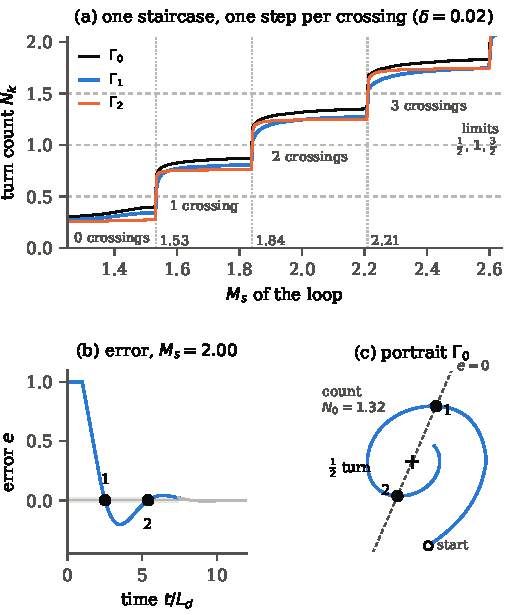
\includegraphics[width=\columnwidth]{fig_stair.pdf}
\caption{What a turn count is, on the lag-cancelled loop. (a) The three
counts against $M_s$ form one staircase, one step per setpoint crossing
(steps at the values of Table~\ref{tab:cert}); the limits
$\frac12,1,\frac32$ (dashed) lie in the gaps. (b) A record with
$M_s=2.00$ crosses twice before it settles within $\delta$. (c) Its
portrait $\Gamma_0$: between the crossings (on the dashed line $e=0$) the
curve turns exactly half a turn around the end point ($+$). The radius is
compressed for visibility; the angle is not.}
\label{fig:stair}
\end{figure}

\subsection{Low counts can hide a high peak}

Outside lag-cancelled loops, crossings and $M_s$ come apart in both
directions. Take a first-order plant with $T=0.3L_d$ and PI with slow integral action,
$T_i=8T$, and $K_c$ set for a gain margin of $1.62$. The error never
crosses the setpoint by more than $2\%$. The two counts that \spin uses
for PI stay below $0.1$ turn. Yet $M_s=2.62$. The oscillation rides on a
slow decay that does not change sign. Only $\Gamma_2$, which \spin does not
use for PI, sees it ($N_2=4.2$). Conversely, on $e^{-s}/(20s+1)$ with PI
($K_c=2.5$, $T_i=5$), the error crosses twice with $26\%$ overshoot, yet
$M_s=1.34$: the overshoot comes from the controller zero. In a grid of
$630$ first-order loops with $T/L_d\le5$, two or more crossings did mean
$M_s\ge1.69$, but this is a tendency, not a bound. % [NEW]
So in general the counts can guide tuning but cannot certify it. Yet the
same step still shows the peak
(Fig.~\ref{fig:record}(a)); Section~\ref{sec:record} explains why.
% [NEW] fig_record.py, reproduce.py --grid

\section{Result 2: The Same Step Gives $M_s$}
\label{sec:record}

\begin{lemma}[One-step certificate]
\label{thm:record}
Let the loop be linear, time invariant, stable and of one degree of
freedom. Let $e$ be the error after a unit setpoint step, and $E$ its
Fourier transform. Then
\begin{equation}
S(j\omega)=j\omega\,E(j\omega)
=1+\int_0^\infty\dot e(t)\,e^{-j\omega t}\,dt.
\label{eq:srecord}
\end{equation}
So $M_s=\max_\omega|S(j\omega)|$ follows from the record, and $L=1/S-1$
gives the gain and phase margins.
\end{lemma}

\begin{proof}
With $R=1/s$ the transform of the step, $E=R/(1+L)=RS$, so
$S=sE$. The error jumps from $0$ to $1$ at $t=0$. This
jump gives the constant term.
\end{proof}

We call the value read by \eqref{eq:srecord} the certificate. Inside
\spin, it becomes the acceptance test of Section~\ref{sec:spin}.
The identity is exact. Any error in the reading comes from sampling, from
noise, or from a record that has not settled. We computed the exact
record of the loop \eqref{eq:loop} from its Lambert series. The peak read
by \eqref{eq:srecord} equals the true value $M_s=2.23222$ to all five
digits. On a zero-order-hold simulation of plant $P_4$
(Section~\ref{sec:spin}) with SIMC PI, the reading error falls from $0.39\%$ at $25$
samples per dead time to $0.05\%$ at $100$ samples. % [NEW]
A real controller is also sampled. The record then gives the $M_s$ of the
loop that actually runs. Fig.~\ref{fig:record}(b) shows the reading
error on all loops of this paper. It is between $-0.8\%$ and $+0.8\%$
for the reference loops and for every tuning that certified \spin
accepted, and between $-0.8\%$ and $+1.3\%$ for the sharper peaks of the
tunings that original \spin accepted. % [NEW] fig_record.py

\begin{corollary}[Two degrees of freedom]
\label{cor:2dof}
Let the controller be $u=C_rr-C_{fb}y$, for example with setpoint
weighting or with the derivative on the measurement. Let $C_{fb}$ be
known. Then, from the recorded $u$ and $y$ of one setpoint step,
\begin{equation}
G(j\omega)=\frac{\int_0^\infty\dot y\,e^{-j\omega t}dt}
{\int_0^\infty\dot u\,e^{-j\omega t}dt},\qquad
S=\frac{1}{1+C_{fb}G},
\label{eq:2dof}
\end{equation}
where $\dot u$ includes the jump of $u$ at $t=0$.
\end{corollary}

\begin{proof}
$Y=GU$, so $sY/(sU)=G$. In a stable loop both derivatives decay
exponentially, so their transforms exist. The loop transfer function is
$C_{fb}G$.
\end{proof}

We tested both forms on the plants of Section~\ref{sec:spin} with SIMC
PID, sampled as in Section~\ref{sec:spin}. For a one-degree-of-freedom
loop, both forms are within $0.5\%$ of the true $M_s$. With setpoint
weight $b=0$ and the derivative on the measurement, the simple form
$j\omega E$ is wrong by $-14\%$ to $+8\%$, while form \eqref{eq:2dof}
stays within $0.2\%$ on all four plants. Noise biases the ratio of two
noisy transforms in \eqref{eq:2dof}; our noise test below covers only
the simple form. % [NEW] twodof.py (controller sampled at T_f/20)

\begin{figure*}[t]
\centering
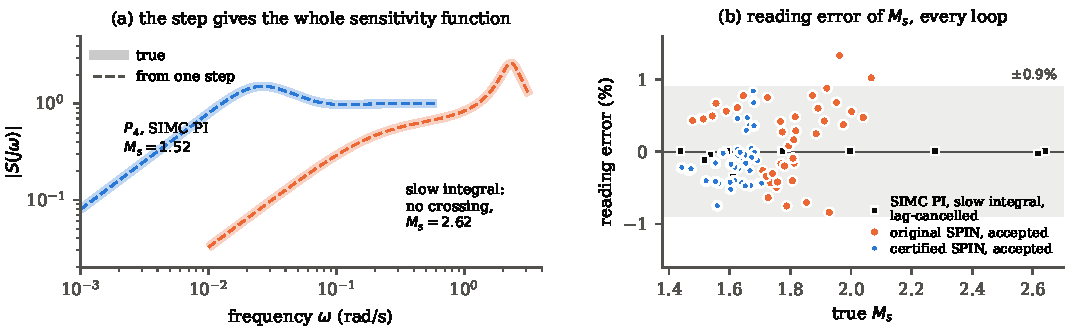
\includegraphics[width=0.92\textwidth]{fig_record.pdf}
\caption{Lemma~\ref{thm:record}. (a) $|S|$ from one setpoint step
(dashed) lies on the true one (thick), for $P_4$ with SIMC PI and for the
slow-integral loop whose peak the counts miss. (b) Reading error of all
$122$ readings: $11$ reference loops (SIMC PI on $P_1$--$P_4$, the
slow-integral loop, the lag-cancelled loop for $k=0.4,\dots,0.9$) and the
$111$ distinct tunings accepted by original ($69$) or certified ($42$)
\spin in Section~\ref{sec:spin}; the band is $\pm0.9\%$.}
\label{fig:record}
\end{figure*}

\paragraph*{Noise} White noise on the record biases the reading up, to
the safe side. Over $20$ records on each of the four plants, $1\%$ noise
gave a bias of $+0.1$ to $+0.6\%$ (spread ${<}0.6\%$), and $5\%$ noise
$+1.3$ to $+4.9\%$ (spread ${<}2.5\%$). % [NEW] noise.py

\paragraph*{Conditions} The record must settle; otherwise the tail must
be treated as in \cite{WangHangBi1997}. The sampling must be fast enough
for the crossover frequency and for any derivative filter. The step must
stay in the linear range, without actuator saturation.

\section{Certified \spin}
\label{sec:spin}

\paragraph*{The limits are half-turn limits} After whitening each
portrait with its second-moment matrix, a single oscillation gives three
equal counts on the half turns of Section~\ref{sec:count}
(Fig.~\ref{fig:stair}), and the limits $\bar N=(\tfrac12,1,\tfrac32)$ lie
in the gaps. The per-axis limits $(0.5,0.75,1.0)$ of \spin separate the
same $0|1$, $1|2$ and $2|3$ crossings: on the lag-cancelled loop the
per-axis counts lie in $[0.06,0.25]$, $[0.55,0.74]$ and $[1.03,1.24]$,
those of $\Gamma_2$ half a turn lower. The limits make the count decisions
robust, not the tuning. % [NEW] lagcancel.py + compare.counts_old

\paragraph*{Acceptance test} When no count is above its limit, \spin
would raise all gains (line 7 of Algorithm~1). Algorithm~2 first reads
$\hat M_s$ and its frequency $\omega_p$ from the same record by
Lemma~\ref{thm:record}. If $\hat M_s\le M^*$, the tuning is accepted. If
not, the same record also tells which gain to lower, because it gives the
loop $L=1/S-1$ and so the sensitivity of any other tuning of the same
plant.

\begin{proposition}[Shaping from one step]
\label{prop:shape}
Let $C$ be a PID controller with gains $K_k$ ($k=i,p,d$, the
bands $\Gamma_0,\Gamma_1,\Gamma_2$; the derivative filter is tied to $K_d/K_p$), let $S$ be read from the step, and
let $\omega_p$ be the unique peak of $|S|$, $M=|S(j\omega_p)|$,
$T=1-S$, $c_k=K_k\,\partial C/\partial K_k$.
\begin{enumerate}
\item[(a)] $g_k=\partial\ln M/\partial\ln K_k=-\mathrm{Re}\,(T c_k/C)$ at
$\omega_p$, and $\sum_k g_k=\mathrm{Re}\,S(j\omega_p)-1$.
\item[(b)] Lowering all gains lowers $M$ to first order iff
$\mathrm{Re}\,S(j\omega_p)>1$, that is iff $|L+\tfrac12|<\tfrac12$ at
$\omega_p$.
\item[(c)] \spin's move for band $k$ (lower $K_k$, raise the bands below,
all by the same factor) lowers $M$ to first order iff
$g_k>\sum_{j<k}g_j$. If $\sum_kg_k>0$, such a band always exists.
\item[(d)] For any other controller $C'$ the sensitivity is
$S'=1/(1+LC'/C)$, exactly, with $L=1/S-1$.
\end{enumerate}
\end{proposition}

\begin{proof}
(a) $\partial\ln S/\partial\ln K_k=-(c_k/C)\,L/(1+L)=-Tc_k/C$ and
$\ln M=\mathrm{Re}\ln S$ at the peak; the $c_k$ add up to $C$, so
$\sum g_k=-\mathrm{Re}\,T$. (b) is $\sum g_k>0$; and
$\mathrm{Re}\,\frac1{1+L}>1\Leftrightarrow 1+\mathrm{Re}\,L>|1+L|^2
\Leftrightarrow|L+\tfrac12|^2<\tfrac14$. (c) The move changes $\ln M$ by
$\ln\frac1{1-\beta}\,(\sum_{j<k}g_j-g_k)$. Let $P_k=\sum_{j\le k}g_j$.
The condition is $P_k>2P_{k-1}$. If $\sum_kg_k>0$, take the smallest $k$ with
$P_k>0$: then $P_{k-1}\le0$ and the condition holds. (d) $L'=LC'/C$ for
the same plant.
\end{proof}

Three cautions apply. The first-order sign in (a)--(c) is wrong for about
$1$--$2\%$ of finite $10\%$ steps, so Algorithm~2 uses (d), exact up to
the reading error amplified by $T'/T$. $\mathrm{Re}\,S>1$ fails for about $1\%$ of
loops with strong integral action. And (d) predicts a frequency response,
not stability; the next step checks it. On $934$ moves of our runs
with $\mathrm{Re}\,S>1$ and a unique peak, the condition held every
time, the prediction was within $1.2\%$ of the true $M_s$, and the true
$M_s$ fell in $99$--$100\%$ of them. % [NEW] designed.py shape_move, analyze_shape.py

\begin{figure}[t]
\small
\hrule\smallskip
\noindent\textbf{Algorithm 2:} certified \spin: line 7 of Algorithm~1
becomes
\smallskip\hrule\smallskip
\noindent\begin{tabular}{@{}r@{\hspace{0.6em}}l@{}}
7a: & read $\hat M_s$, $\omega_p$ and $L=1/S-1$ from the same
record\\
7b: & \textbf{if} $\hat M_s\le M^*$ \textbf{then} raise all
gains by one step \hfill (accept)\\
7c: & \textbf{else for each} band $k$: predict $M_s$ after \spin's
move\\
    & for band $k$ by Prop.~\ref{prop:shape}(d)\\
7d: & apply the \emph{highest} band whose predicted $M_s$ is below
$\hat M_s$;\\
    & if none, lower all gains; continue at line 10\\
\end{tabular}
\smallskip\hrule\smallskip
\noindent Default $M^*=1.7$. Every accepted tuning then has
$M_s\le M^*$, up to the reading error.
\smallskip\hrule
\end{figure}

Any band predicted to help reaches the target; we take the highest
because it left the lower bands, which carry the load rejection, largest
(see below). In Fig.~\ref{fig:certified}(b),
$P_3$ with PID, the step of the tuning that original \spin accepts reads
$\hat M_s=1.81$ with $g=(0.44,0.41,-0.05)$; lowering $K_i$ is predicted to
give $1.739$ and does give $1.742$.

\paragraph*{Test} We compare original \spin, exactly as published,
with certified \spin, which adds only Algorithm~2 with $M^*=1.7$.
Both run for $200$ iterations, filter the derivative with ratio $10$, and
keep each gain within $[0.001,10]$ times its start value \cite{SPIN}.
Because this box ties the result to the start, we run every loop from two
starts: SIMC on a half-rule model with $\tau_c=3\theta$, and a start
twice as bold ($\tau_c=\theta$). The plants are the four plants of \cite{SPIN},
\begin{align*}
P_1&=\frac{e^{-s}}{(10s+1)(s+1)^3}, &
P_2&=\frac{1.25\,e^{-8s}}{(5s+1)^4},\\
P_3&=\frac{e^{-10s}}{(2s+1)(s+1)^3}, &
P_4&=\frac{e^{-4s}}{(8s+1)^6},
\end{align*}
with PI and PID. Four more plants place the oscillation in a
chosen band: a delay-dominant $e^{-5s}/(s+1)$ and two lag-dominant plants,
$e^{-s}/(10s+1)$ and $e^{-0.5s}/((10s+1)(s+1))$, with PI, and a fast plant
$e^{-0.1s}/((s+1)(0.5s+1))$ with PID. We also use the family
$e^{-L_ds}/((s+1)(0.5s+1)(0.25s+1))$ with PID and
$L_d\in\{0.25,0.5,1,2,4,8,16\}$, so that the dead-time share
$L_d/(L_d+\sum T)$ runs from $0.125$ to $0.90$. At the end, \spin moves in
a cycle between a few tunings. We report the most aggressive tuning that
each rule accepts in its last $60$ iterations. The controller is sampled at $1/20$ of the derivative filter time
constant (PID) or $1/1000$ of the plant's time scale (PI). % [NEW] designed.py

\begin{table}[t]
\centering
\caption{True $M_s$ of the most aggressive tuning that original and
certified \spin accept, from the cautious ($3\theta$) and the bold
($\theta$) start; the band that owns the peak of the original tuning from
the cautious start; and the change of load-step IAE there.}
\label{tab:spin}
\small\setlength{\tabcolsep}{3.2pt}
\begin{tabular}{llcccccc}
\toprule
& & \multicolumn{2}{c}{original} & \multicolumn{2}{c}{certified} & & \\
\cmidrule(lr){3-4}\cmidrule(lr){5-6}
& & $3\theta$ & $\theta$ & $3\theta$ & $\theta$ & owner & $\Delta$IAE \\
\midrule
$P_1$ & PI  & $1.47$ & $1.47$ & $1.47$ & $1.47$ & $\Gamma_1$ & -- \\
      & PID & $1.67$ & $\mathbf{1.85}$ & $1.67$ & $1.62$ & $\Gamma_1$ & -- \\
$P_2$ & PI  & $1.64$ & $1.67$ & $1.64$ & $1.67$ & $\Gamma_1$ & -- \\
      & PID & $1.60$ & $\mathbf{1.78}$ & $1.60$ & $1.66$ & $\Gamma_1$ & -- \\
$P_3$ & PI  & $1.67$ & $1.63$ & $1.67$ & $1.63$ & $\Gamma_0$ & -- \\
      & PID & $\mathbf{1.81}$ & $\mathbf{1.74}$ & $1.69$ & $1.67$ & $\Gamma_1$ & $+24\%$ \\
$P_4$ & PI  & $1.55$ & $1.60$ & $1.55$ & $1.60$ & $\Gamma_1$ & -- \\
      & PID & $1.62$ & $1.56$ & $1.62$ & $1.56$ & $\Gamma_1$ & -- \\
\midrule
delay-dom. & PI & $1.68$ & $1.63$ & $1.68$ & $1.63$ & $\Gamma_0$ & -- \\
lag-dom.   & PI & $\mathbf{2.00}$ & $1.68$ & $1.67$ & $1.68$ & $\Gamma_1$ & $+52\%$ \\
2 lags     & PI & $1.44$ & $1.47$ & $1.44$ & $1.47$ & $\Gamma_1$ & -- \\
fast & PID & $\mathbf{1.87}$ & $\mathbf{1.97}$ & $1.66$ & $1.68$ & $\Gamma_2$ & $0\%$ \\
\bottomrule
\end{tabular}
\end{table}
% [NEW] designed.py with SPIN_BOX=1 (START_SCALE=1,2), RULES_ONLY=original+shape-hi (shapehi*.jsonl), owner_designed.py (OWN_IN=box), analyze_shape2.py

\begin{figure*}[t]
\centering
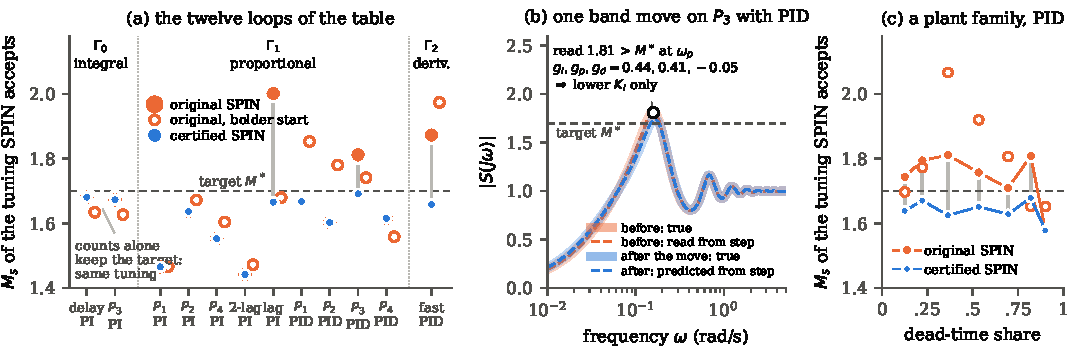
\includegraphics[width=\textwidth]{fig_certified.pdf}
\caption{Original against certified \spin ($M^*=1.7$). (a) The loops of
Table~\ref{tab:spin}, grouped by the band that owns the peak of the
original tuning. Filled orange: original, cautious start; open orange:
original, bold start; blue: certified, cautious start. (b) One band move
on $P_3$ with PID: the step reads $1.81>M^*$ at $\omega_p$ ($\circ$), the
gradient of Proposition~\ref{prop:shape} picks $K_i$, and the sensitivity
predicted from the same step lies on the true one after the move. (c) The
family $e^{-L_ds}/((s+1)(0.5s+1)(0.25s+1))$ with PID against the
dead-time share.}
\label{fig:certified}
\end{figure*}

\paragraph*{Where the oscillation is decides} Original \spin ended above
the target on $9$ of the $19$ loops from the cautious start (up to
$M_s=2.00$) and on $8$ from the bold start (up to $2.07$). In most PID
runs the derivative gain ended at the ceiling of the box, so the box set
the result and which loops failed depended on the start ($P_1$ and $P_2$
with PID passed from the cautious start and failed from the bold one; the
lag-dominant PI loop did the opposite). Every failure was owned by $\Gamma_1$ or $\Gamma_2$. The
three loops owned by $\Gamma_0$ (delay-dominant PI, $P_3$ with PI, and the
family at $L_d=16$) stayed below the target from both starts; there the
counts alone suffice. Certified \spin ended at or below the target on all
$19$ loops from both starts. The highest true value was $M_s=1.705$, read
as $1.697$. On the plant family (Fig.~\ref{fig:certified}(c)), original
\spin exceeded the target at every dead-time share up to $0.82$ ($M_s$
from $1.71$ to $1.81$; from the bold start up to $2.07$ at $L_d=1$), and
certified \spin stayed between $1.58$ and $1.68$.

\paragraph*{Which part does the work} Without the box, the counts alone
Original \spin then went above the target on all $11$ PID loops
that converged (all but $L_d=16$), up to $M_s=2.04$. Certified \spin ended
at or below $1.705$ on all of them (read $1.698$ at most), so the target
does not rely on any gain bound.
% [NEW] designed.py (no box), RULES_ONLY=original,original+shape-hi (nbshape*.jsonl)

\paragraph*{The price} A lower peak costs load rejection. For a unit load
step at the plant input, the integrated absolute error (IAE) of the
cautious start rose by $0$ to $15\%$ on six of the nine loops whose tuning
Algorithm~2 changed, by $24\%$ on two, and by $52\%$ on the lag-dominant PI
loop; the fast PID loop, which original \spin tuned to $M_s=1.87$,
lost nothing. The mean over all $19$ loops was $+7.7\%$ (bold start:
$+5.1\%$). Choosing the band by the largest term of $|C|$ instead cost
$+11.1\%$, and $+88\%$ on the fast loop. % [NEW] analyze_shape2.py


\section{Use in Practice}
\label{sec:practice}

\emph{By eye,} on a lag-cancelled loop: count how often the error
crosses the setpoint before it stays within $2\%$. A SIMC loop crosses
once; with $\lambda\ge(e-1)L_d$ lambda tuning never crosses
(Proposition~\ref{prop:cross}(a)). \emph{By computer:} every setpoint
change in a historian gives $M_s$ and the margins by
Lemma~\ref{thm:record} or Corollary~\ref{cor:2dof}, without a model.

\emph{Scope:} this paper stays in theory and simulation: $19$ simulated
loops, two starts, the conditions of Section~\ref{sec:record}. As in
\cite[Remark~2]{SPIN}, the counts assume noise below about $2\%$ of the
step. Noise in the counts and real loops are the subject of a follow-up.
Scripts that reproduce every number and figure are in the repository
\url{https://github.com/ottapav/robopid-simulator}, folder
\texttt{docs/ECC27\_certified\_SPIN}.

\section{Conclusion}

The results are twofold. On lag-cancelled loops a \spin count has an
exact meaning: half a turn per setpoint crossing, and the calibrated
limits separate crossing numbers. On any other stable loop, counts and
$M_s$ are not tied, but the step that \spin already records gives the
peak and the loop, because its error is the step response of the
sensitivity function. As an acceptance test with band shaping, it turned
a start-dependent result (about half of our loops above the target) into
a certified one (all loops at the target, within the reading error), at a
mean cost of $5$ to $8\%$ in load rejection. A follow-up will study
noise and real loops.

{\small
\begin{thebibliography}{99}

\bibitem{SPIN} D.~Pachner, P.~Otta, J.~Dost\'al, and V.~Havlena,
``Model-free PID tuning by step-response inspection,'' submitted to
\emph{J. Process Control}, 2026.

\bibitem{AstromHagglund2004} K.~J.~\r{A}str\"om and T.~H\"agglund,
``Revisiting the Ziegler--Nichols step response method for PID control,''
\emph{J. Process Control}, vol.~14, no.~6, pp.~635--650, 2004.

\bibitem{Skogestad2003} S.~Skogestad, ``Simple analytic rules for model
reduction and PID controller tuning,'' \emph{J. Process Control},
vol.~13, no.~4, pp.~291--309, 2003.

\bibitem{SkogestadGrimholt2012} S.~Skogestad and C.~Grimholt, ``The SIMC
method for smooth PID controller tuning,'' in \emph{PID Control in the
Third Millennium}, R.~Vilanova and A.~Visioli, Eds. London: Springer,
2012, pp.~147--175.

\bibitem{Desborough2002} L.~Desborough and R.~Miller, ``Increasing
customer value of industrial control performance monitoring---Honeywell's
experience,'' in \emph{Chemical Process Control VI}, AIChE Symp. Ser.
no.~326, vol.~98, 2002, pp.~169--188.

\bibitem{Bauer2016} M.~Bauer, A.~Horch, L.~Xie, M.~Jelali, and
N.~Thornhill, ``The current state of control loop performance
monitoring---a survey of application in industry,'' \emph{J. Process
Control}, vol.~38, pp.~1--10, 2016.

\bibitem{WangHangBi1997} Q.-G.~Wang, C.~C.~Hang, and Q.~Bi, ``Process
frequency response estimation from relay feedback,'' \emph{Control Eng.
Pract.}, vol.~5, no.~9, pp.~1293--1302, 1997.

\bibitem{VandenHofSchrama1993} P.~M.~J.~Van den Hof and
R.~J.~P.~Schrama, ``An indirect method for transfer function estimation
from closed loop data,'' \emph{Automatica}, vol.~29, no.~6,
pp.~1523--1527, 1993.

\bibitem{Isoshima2023} K.~Isoshima, M.~Tanemura, and Y.~Chida,
``Data-driven estimation of the lower bounds of gain and phase margins,''
\emph{Automatica}, vol.~153, art.~111008, 2023.

\bibitem{AslUlsoy2003} F.~M.~Asl and A.~G.~Ulsoy, ``Analysis of a system
of linear delay differential equations,'' \emph{J. Dyn. Syst. Meas.
Control}, vol.~125, no.~2, pp.~215--223, 2003.

\bibitem{GyoriLadas1991} I.~Gy\H{o}ri and G.~Ladas, \emph{Oscillation
Theory of Delay Differential Equations with Applications}. Oxford:
Clarendon Press, 1991.

\bibitem{IFT1998} H.~Hjalmarsson, M.~Gevers, S.~Gunnarsson, and
O.~Lequin, ``Iterative feedback tuning: theory and applications,''
\emph{IEEE Control Syst. Mag.}, vol.~18, no.~4, pp.~26--41, 1998.

\bibitem{Killingsworth2006} N.~J.~Killingsworth and M.~Krsti\'c, ``PID
tuning using extremum seeking: online, model-free performance
optimization,'' \emph{IEEE Control Syst. Mag.}, vol.~26, no.~1,
pp.~70--79, 2006.

\bibitem{Shamsuzzoha2010} M.~Shamsuzzoha and S.~Skogestad, ``The setpoint
overshoot method: a simple and fast closed-loop approach for PID tuning,''
\emph{J. Process Control}, vol.~20, no.~10, pp.~1220--1234, 2010.

\bibitem{VRFT2002} M.~C.~Campi, A.~Lecchini, and S.~M.~Savaresi,
``Virtual reference feedback tuning: a direct method for the design of
feedback controllers,'' \emph{Automatica}, vol.~38, no.~8,
pp.~1337--1346, 2002.

\end{thebibliography}}

\end{document}
